\documentclass{beamer}
\mode<presentation>

\usepackage{color}
\usepackage{tikz}
\usepackage{multimedia}
\usetikzlibrary{arrows,chains,matrix,positioning,scopes}

% \usetheme{Warsaw} NOOOOOOOOOOOO
% \usecolortheme{rose}
\usecolortheme{seahorse}
% \usefonttheme[onlylarge]{structuresmallcapsserif}


% \setbeamersize{sidebar width right=5cm}
% \setbeamertemplate{section in sidebar}{section in sidebar}




% \defbeamertemplate*{title page}{customized}[1][]
% {
%   \usebeamerfont{title}\inserttitle\par
%   \usebeamerfont{subtitle}\usebeamercolor[fg]{subtitle}\insertsubtitle\par
%   \bigskip
%   \usebeamerfont{author}\insertauthor\par
%   \usebeamerfont{institute}\insertinstitute\par
%   \usebeamerfont{date}\insertdate\par
%   \usebeamercolor[fg]{titlegraphic}\inserttitlegraphic
% }

\title{Monitoraggio in tempo reale delle apnee respiratorie del sonno
attraverso uno stetoscopio elettronico}
% \subtitle{Monitoraggio della respirazione attraverso uno stetoscopio elettronico}
\author{Federico Viscomi}
\date{20 Marzo 2013}
% \date{\today}

%  \usetheme{beamerTheme}
\setbeamertemplate{footline}[page number]{}

\setbeamertemplate{navigation symbols}{}




\begin{document}


\begin{frame}
\titlepage
\end{frame}


\begin{frame}
\frametitle{Outline}
\tableofcontents
\end{frame}




\section{Obiettivi}
\begin{frame}
  \frametitle{Obiettivi}
    Progettare, prototipare e valutare un software di riconoscimento in tempo reale delle apnee respiratorie nel sonno attraverso uno stetoscopio elettronico applicato sul petto di un soggetto.
%           Esponi appena possibile (scrivendolo esplicitamente su una slide) l’obiettivo del lavoro e l’idea che lo rende interessante, il valore aggiunto, il contributo originale. 
% Non addentrarti in nessuna spiegazione prima di aver comunicato a chi ti ascolta “dove stai andando”.
\end{frame}
    


\section{Apnea}

\begin{frame}
\frametitle{Cos'\`e una apnea?}

\begin{itemize}
  \item
    \textcolor{blue}{Respirazione}
  \item
    \textcolor{blue}{Fasi respiratorie}: inspirazione, espirazione e pausa respiratoria.
  \item
    \textcolor{blue}{Apnea}: pausa respiratoria di durata uguale o maggiore di $10s$.
\end{itemize}

% \begin{definition}
% Una \alert{apnea} \`e una 
% \end{definition}
\end{frame}

\begin{frame}
  \frametitle{Sindrome da apnea del sonno}
\subsection{Sindrome da apnea del sonno}
\begin{center}
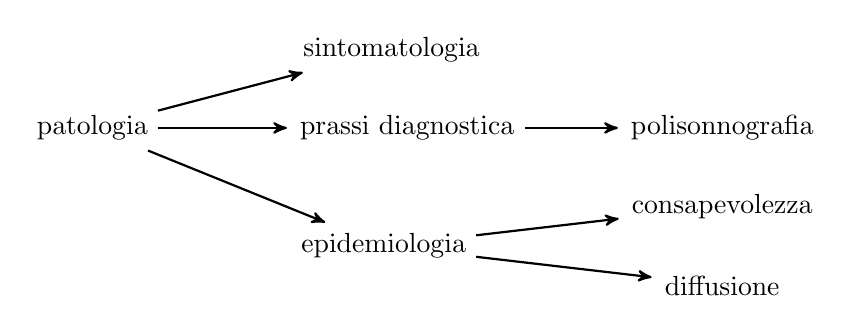
\begin{tikzpicture}
%   [scale=.8,auto=left,every node/.style={fill=blue!20}]
[->,>=stealth',shorten >=1pt,auto,node distance=3cm,
  thick,main node/.style={circle,fill=blue!20,draw,font=\sffamily\Large\bfseries}]


  \node (patologia) at 			(0,2) 	{patologia};

  \node (epidemiologia) at 		(3.7,0.5)		{epidemiologia};
  \node (diagnosi) at 			(4,2) 		{prassi diagnostica};
   \node (sintomatologia) at 		(3.8,3) 		{sintomatologia};


  \node (polisonnografia) at 		(8,2) 	{polisonnografia};
  \node (diffusione) at 		(8,0) 		{diffusione};
  \node (consapevolezza) at 		(8,1) 		{consapevolezza};


   \foreach \from/\to in {patologia/sintomatologia,patologia/epidemiologia,patologia/diagnosi,diagnosi/polisonnografia, epidemiologia/diffusione, epidemiologia/consapevolezza}
     \draw (\from) -- (\to);

\end{tikzpicture}
\end{center}
\end{frame}



\section{Motivazione}
  \subsection{Diagnosi e terapia d'emergenza}


  \begin{frame}
  \frametitle{Motivazione}
\endcenter

% \begin{description}
%   \item[Diagnosi]: Utile di per s\'e. Meno invasiva. Meno costosa.
%   \item[Terapia d'emergenza]:
%     Svegliare il soggetto. Come scegliere la soglia di allarme? Conviene svegliare il soggetto?
% \end{description}
% \begin{flushleft}
\begin{itemize}
 \item[] 
    \textcolor{blue}{Diagnosi}

    Utile di per s\'e. Meno invasiva. Meno costosa.
 \item[]
  \textcolor{blue}{Terapia d'emergenza}

  Svegliare il soggetto. Come scegliere la soglia di allarme? Conviene svegliare il soggetto?
\end{itemize}
% \end{flushleft}



% \begin{tikzpicture}
% %   [scale=.8,auto=left,every node/.style={fill=blue!20}]
% [->,>=stealth',shorten >=1pt,auto,node distance=3cm,
%   thick,main node/.style={circle,fill=blue!20,draw,font=\sffamily\Large\bfseries}]
% 
%   \node (diagnosi) at 		(0,2) 	{diagnosi};
%   \node (terapia) at 		(0,4) 	{terapia d'emergenza};
%   \node (utile) at 		(4,1.5) {utile di per se};
%   \node (menoInvasiva) at 	(4,2) 	{meno invasiva};
%   \node (economica) at 		(4,2.5) {pi\`u economica};% di una polisonnografia classica
%   \node (svegliare) at 		(4,4) 	{svegliare il soggetto};
%   
% 
%    \foreach \from/\to in {diagnosi/utile,terapia/svegliare,diagnosi/menoInvasiva,diagnosi/economica}
%      \draw (\from) -- (\to);
% 
% \end{tikzpicture}
\end{frame}


    
% La sindrome da apnea del sonno \`e una patologia molto diffusa. 
% Il sonno di un soggetto affetto da tale patologia \`e disturbato da apnee e da episodi di respirazione insufficiente. 
% Forme medie e gravi di sindrome da apnea del sonno sono un fattore di rischio per, e una concausa di: pressione alta, malattie cardiache, diabete, depressione. 
% Inoltre tale patologia contribuisce a creare una senso perenne di sonnolenza e spossatezza. 
% Si stima che pi\`u della met\`a dei soggetti affetti da tale patologia non ne siano al corrente\cite{intrrr}. 
% Questo a causa dei meccanismi di diagnosi pi\`u diffusi che sono costosi o scomodi e richiedono al paziente di trascorrere la notte in un centro specializzato.
% Inoltre i centri specializzati sono pochi e possono essere molto costosi. 
% Sono in fase di sviluppo ma non hanno per il momento una diffusione capillare altri strumenti di diagnosi pi\`u pratici. 
% Alcuni studi hanno analizzato i dati di alcuni soggetti che sono morti a causa di eventi cardiovascolari acuti e che erano 
% affetti da forme medie o gravi di sindrome da apnea del sonno. 
% La conclusione \`e stata che la maggior parte di tali soggetti \`e morta durante il sonno. 
% In questa tesi sviluppiamo un prototipo di uno strumento non invasivo di monitoraggio del respiro e di diagnosi della sindrome da apnea del sonno: attraverso uno stetoscopio elettronico, il sistema deve vigilare su un soggetto e registrare la frequenza e la durata delle apnee e, cosa pi\`u importante, deve svegliare il soggetto nel caso in cui l'apnea duri troppo. 


\subsection{Svegliare il soggetto}
\begin{frame}
    \frametitle{Conviene svegliare il soggetto?}
    \framesubtitle{Motivi empirici\footnote{\emph{Day–Night Pattern of Sudden Death in Obstructive Sleep Apnea.} 
  	Apoor S. Gami, Daniel E. Howard, Eric J. Olson, and Virend K. Somers.
  	The new england journal of medicine.} e biologici}
\begin{center}
\begin{figure}
 \includegraphics[height=0.65\textheight]{./daynight2.png}
 % daynight.xcf: 566x589 pixel, 72dpi, 19.97x20.78 cm, bb=0 0 566 589
\end{figure}
\end{center}
% non dice che i soggetti hanno una apnea immediatamente prima di morire, per questo c'e' bisogni di ulteriori esperimenti fatti da una equipe medica

\end{frame}

% \begin{frame}
%     \frametitle{Conviene svegliare il soggetto?}
%     \framesubtitle{Motivi biologici}
% 
% % \begin{itemize}
% % \item 2 is prime (two divisors: 1 and 2).
% % \pause
% % \item 3 is prime (two divisors: 1 and 3).
% % \pause
% % \item 4 is not prime (\alert{three} divisors: 1, 2, and 4).
% % \end{itemize}
% 
% \end{frame}
% 



% \subsection{Scelta della soglia}
% \begin{frame}
%   \frametitle{Scelta della soglia}
% \begin{tikzpicture}
% [->,>=stealth',shorten >=1pt,auto,node distance=3cm, thick,main node/.style={circle,fill=blue!20,draw,font=\sffamily\Large\bfseries}]
% \node (soglia) at (0,1.5) {soglia di allarme};
% \node (apnea) at (3.7,3) {definizione di apnea};
% \node (ipossiemia) at (4,1) {ipossiemia};
% \node (tradeoff) at (3.8,2) {trade off};
% \node (variabile) at (3.4, 0) {variabile};
% 
%    \foreach \from/\to in {soglia/tradeoff,soglia/apnea,soglia/ipossiemia, soglia/variabile}
%       \draw (\from) -- (\to);
% \end{tikzpicture}
% \end{frame}


\chapter{Analisi delle Metodologie}


In generale un sistema che riconosce la respirazione a partire da alcuni segnali fisiologici continui, deve essere sensibile al cambiamento di alcune caratteristiche del segnale che sono omomorfe alla presenza, al volume, al flusso o alla frequenza della respirazione. 
Queste caratteristiche sono in generale dipendenti dal contesto quindi ci aspettiamo che un buon algoritmo faccia leva su delle quantit\`a statistiche del segnale o su una qualche forma di apprendimento automatico. 
Ci aspettiamo anche che tali caratteristiche rispettino un qualche principio di localit\`a questo perch\'e le propriet\`a della respirazione cambiano molto nel lungo termine.

La figura \ref{schemaGeneraleAlg} mostra uno schema generale nel quale rientrano tutti i possibili sistemi software di riconoscimento della respirazione attraverso dei sensori.
\begin{figure}[!b]
 \centering
 \includegraphics{./metodologiaDiagramma.png}
 % metodologiaDiagramma.png: 504x232 pixel, 96dpi, 13.33x6.14 cm, bb=0 0 378 174
  \caption{Schema generale di un software di riconoscimento della respirazione}
  \label{schemaGeneraleAlg}
\end{figure}


\section{Metodo elementare}
Siamo tentati dal dire che per risolvere il problema \`e sufficiente l'algoritmo \ref{algoritmoElementare}. 
Anche nelle ipotesi che non ci sia alcun rumore ambientale, non abbiamo la certezza che tale algoritmo funzioni per via di altri rumori fisiologici che potrebbero essere rilevati dallo stetoscopio ad esempio suoni cardiovascolari, suoni gastrointestinali e muscolari. 
L'algoritmo tuttavia \`e sottospecificato in quanto ci sono vari gradi di libert\`a: la scelta della soglia e la scelta della dimensione della finestra. 
Dai dati disponibili nella letteratura riguardo i suoni registrati da uno stetoscopio non siamo in grado di dire se possiamo scegliere i parametri dell'algoritmo in modo da farlo funzionare correttamente.
Riteniamo quindi che almeno un primo livello di trattamento del segnale sia necessario per risolvere questo problema. 
Inoltre una implementazione cos\`i banale \`e probabilmente possibile realizzarla ad un livello pi\`u basso ad esempio direttamente nel firmware dello stetoscopio. 

\incmargin{1em}
\restylealgo{boxed}\linesnumbered
\begin{algorithm}
  \dontprintsemicolon
  \SetVline
  % \SetNoline
%   \SetKwData{b}{b}
%   \SetKwData{This}{this}
%   \SetKwData{Up}{up}
  \SetKwFunction{getAverageLocalEnergy}{getAverageLocalEnergy}
  \SetKwFunction{getInstantSoundEnergy}{getSoundEnergy}
  \SetKwFunction{Write}{write}
  \SetKwFunction{Init}{init}
  \SetKwFunction{Clear}{clear}
  \SetKwFunction{Add}{add}
  \SetKwInOut{Input}{input}
  \SetKwInOut{Output}{output}
  \caption{Naive breath detection}

    \Input{A block of sound samples}
%     \Output{A boolean}
    \BlankLine
%     soundEnergyHistoryBuffer.\Clear{}\;
    \ForEach{window $w$ in the input block}{
      instantSoundEnergy $\leftarrow$ w.\getInstantSoundEnergy{}\;
%       averageLocalEnergy $\leftarrow$ soundEnergyHistoryBuffer.\getAverageLocalEnergy{}\;
%       soundEnergyHistoryBuffer.\Write{instantSoundEnergy}\;
% 			//variance = Util.getVariance(soundEnergyHistoryBuffer, averageLocalEnergy);
% 			// final double linearRegression = Util.getLinearRegression(variance);
% 			//final double linearRegression = 1;
% 			//final boolean isABeat = (instantSoundEnergy > (linearRegression * averageLocalEnergy));
      \eIf{instantSoundEnergy $>$ threshold}{
	is a breath;
% 	beatSequence.\Add{true}\;
% 	breathFrequency $\leftarrow$ (breathFrequency + 1) * (59.0 / 60.0)\;
      }{
	is not a breath;
% 	beatSequence.\Add{false}\;
% 	breathFrequency $\leftarrow$ breathFrequency * (59.0 / 60.0)\;
      }
%     \Return beatSequence\;
  }

\label{algoritmoElementare}
\end{algorithm}
\decmargin{1em}





\section{Beat detection}
La soluzione \`e nata dall'osservazione che il respiro ha un certo ritmo e quindi si pu\`o trattare il respiro come se fosse musica. 
La ricerca sul beat detection ha portato ad una serie di algoritmi e metodi per il trattamento di suoni musicali. 
Da una analisi di questi si capisce che possono essere applicati con opportune modifiche anche ai suoni prodotti dal respiro.




\subsection{Scelta dell'algoritmo}

Secondo \cite{Pekonen} ci sono varie propriet\`a da considerare per scegliere un algoritmo di onset detection. 
Ad esempio: 
\begin{itemize}
  \item
    La complessit\`a dell'algoritmo.
  \item
    Le caratteristiche della piattaforma sulla quale ci si aspetta che l'algoritmo venga usato.
  \item
    La presenza o meno di vincoli sul tempo di esecuzione dell'algoritmo. 
  \item
    Il dominio dell'input: 
    \begin{itemize}
      \item
	Se il segnale ha dei beat molto marcati e presenta relativamente poche voci(ad esempio la musica tecno) allora \`e adeguato un metodo nel dominio del tempo.
      \item
	Se il segnale da analizzare \`e complesso, ad esempio nel caso della musica sinfonica nella quale c'\`e una base di strumenti che fanno da accompagnamento e quindi dettano il ritmo della musica e altri gruppi di strumenti pi\`u legati alla melodia, allora conviene usare un metodo basato su informazione di fase nel dominio delle frequenze, in quanto in questo caso i beat sono legati molto al timbro degli strumenti.
    \end{itemize}
  \item
    Se \`e necessaria una localizzazione precisa nel tempo e nelle frequenze allora si possono usare metodi basati sulle wavelet. 
  \item
    Se la complessit\`a computazionale non \`e un problema ed \`e presente un insieme adatto di segnali di allenamento allora si possono usare metodi basati su apprendimento automatico e informazioni statistiche(reti neurali, support vector machine, modelli nascosti di Markov).
\end{itemize}

Ricordiamo che gli algoritmi di onset detection sono progettati per funzionare su brani musicali. 
Questi possono essere un insieme molto complesso di voci musicali. 
Nel nostro caso le ipotesi sull'input sono pi\`u semplici perch\'e possiamo assimilare il suono registrato dallo stetoscopio sul petto ad un brano musicale composto da due voci: i suoni respiratori e i suoni cardiovascolari. 
Anche nel caso dei suoni tracheali abbiamo due voci: i suoni respiratori e i suoni della deglutizione.
Quindi concludiamo che serve un algoritmo che sfrutta sia una analisi nel dominio delle frequenze che una analisi nel dominio del tempo.



\section{Pattern recognition e apprendimento automatico}
Un'altra possibile soluzione attinge al campo del riconoscimento vocale. 
In particolare alcune tecniche di riconoscimento vocale usano dei classificatori che hanno come mattoni di base i fonemi. 
Il suono della respirazione in un certo senso pu\`o essere pensato come un linguaggio parlato nel quale ci sono solo due tipi di fonemi: l'inspirazione e l'espirazione. 
Sia nel linguaggio parlato che nella respirazione \`e anche importante il riconoscimento del silenzio.
  
\subsection{Reti neurali}
Una soluzione di questo tipo si pu\`o implementare attraverso reti neurali. In generale si pu\`o procedere nel modo seguente:
\begin{enumerate}
  \item 
    Prima di tutto bisogna disporre di un database di registrazioni di suoni respiratori. 
  \item
    I suoni possono attraversare una fase di filtraggio nella quale si rimuove il rumore, si riduce eventualmente la frequenza di campionamento e si cerca di eliminare i suoni cardiovascolari.
  \item
    Questi suoni si segmentano in segmenti di due tipi:
    \begin{itemize}
      \item 
	Suoni che contengono respirazione, cio\`e suoni che contengono il suono prodotto dall'espirazione o dall'inspirazione
      \item
	Suoni che contengono pause respiratorie. 
	Per pause respiratorie in questo caso si intende una pausa in generale e quindi non necessariamente una apnea.
    \end{itemize}
  \item
    Per ogni segmento si calcola una sequenza di $S$ propriet\`a statistiche interessanti ad esempio: la media dei valori assoluti dei coefficienti di Fourier in determinate bande di frequenza; la potenza media dei coefficienti wavelet in determinate bande di frequenza; la deviazione standard dei coefficienti in determinate bande di frequenza; il rapporto tra la media dei valori assoluti in bande di frequenza adiacenti. 
  \item
    Si calcola inoltre la quantit\`a $l$ che \`e la media della durata dei segmenti che contengono suoni respiratori.
  \item
    A questo punto si usano i valori calcolati in precedenza per allenare una rete neurale. 
    Una rete neurale \`e un meccanismo per approssimare una funzione quindi per allenare una rete neurale bisogna fornire ad essa delle coppie $(input,\; output)$. 
    In questo caso possiamo usare due neuroni di output e un un numero di neuroni di input pari ad $n$, dove $n$ \`e il numero di propriet\`a dei segmenti di suono calcolate in precedenza. 
    Possiamo costruire un insieme di allenamento nel modo seguente. 
    Se $S$ \`e una sequenza  relativa ad un segmento di respiro allora inseriamo nell'insieme $(S, (1,0))$ mentre se $S$ \`e una sequenza relativa ad un segmento di pausa inseriamo nell'insieme $(S, (0,1))$. 
  \item	
    Dopo che la rete \`e allenata possiamo usarla per classificare un segnale di input. 
    Come prima cosa si divide il segnale in segmenti di dimensione pari ad $l$
  \item
    Si da il segmento in pasto alla rete neurale; questa produce l'output: $(s,p)$. 
  \item
    Se $s$ \`e maggiore di $p$ allora il segmento \`e un suono; altrimenti \`e una pausa.
\end{enumerate}


\section{Clustering}
% DBSCAN nel quale la distanza tra due punti aumenta con la distanza temporale e diminuisce con il quadrato della y
\label{clusteringMetodologia}

Guardando il grafico della forma d'onda del segnale della respirazione, in assenza di forte rumore, nella giusta scala temporale ed entro certi limiti di quantit\`a temporale del segnale, siamo in grado di dividere il grafico in parti regolari e cicliche e di classificarle in: espirazione, inspirazione, pausa. 
Questo approccio metodologico risulta particolarmente chiaro osservando il grafico in figura \ref{grafico}.

\begin{figure}
\centering
 \includegraphics[width=0.7\textwidth]{./metodologiaImage.jpg}
 % metodologiaImage.xcf: 1366x768 pixel, 72dpi, 48.19x27.09 cm, bb=0 0 1366 768
  \label{grafico}
  \caption{Forma d'onda di un segnale che contiene respiro.}
\end{figure}

Tale processo intuitivo si pu\`o inquadrare nel problema pi\`u generale del clustering. Possiamo procedere nel modo seguente:
\begin{enumerate}
  \item 
    Dividere l'input in blocchi di lunghezza ad esempio $20s$ o in ogni caso un valore abbastanza grande da essere sicuri che ci sia un ciclo respiratorio completo. 
  \item
    Trovare un clustering adatto ai dati di input.
  \item
    Un respiro si pu\`o definire come un cluster di inspirazione seguito da un cluster di espirazione seguito da una pausa. Se il clustering contiene una sequenza di respiri allora il soggetto sta respirando altrimenti no.
\end{enumerate}

Rimane il problema di scegliere l'algoritmo di clustering adatto alla nostra situazione. 
Nel nostro caso siamo di fronte ad un problema di clustering nel quale lo spazio del segnale di input \`e bidimensionale. 
Una dimensione \`e il tempo discreto e l'altra dimensione \`e il valore dei campioni. 
Gli algoritmi di clustering impongono di conoscere a priori il numero di cluster oppure un valore di soglia. 
Una possibilit\`a \`e quella di usare l'algoritmo \ref{determinareClusterN} per determinare il pi\`u probabile numero di cluster. 
In seguito confrontiamo questo valore con il numero di fasi che ci dovrebbero essere in media nel blocco di input analizzato. 
Questo dovrebbe andare bene almeno per il primo blocco. 
Per i blocchi successivi possiamo tenere traccia del numero di cluster e confrontare il valore corrente con i valori passati.

\section{Segnale di input}
% \begin{frame}
%   \begin{example}
%     \frametitle{Esempio di segnale di input.}
%       \begin{center}
%       \begin{figure}
% 	\includegraphics[width=0.9\textwidth]{./normal.png}
% 	% normal.png: 1366x768 pixel, 72dpi, 48.19x27.09 cm, bb=0 0 1366 768
%       \end{figure}
%       \end{center}
%     \movie[label=cells,width=4cm,height=0.5cm,poster,showcontrols,duration=13s]{}{normal.wav}
%   \end{example}
% \end{frame}


\begin{frame}
  \frametitle{Caratteristiche del segnale di input}
  \framesubtitle{Sorgenti sonore del segnale}
  
  \begin{center}
    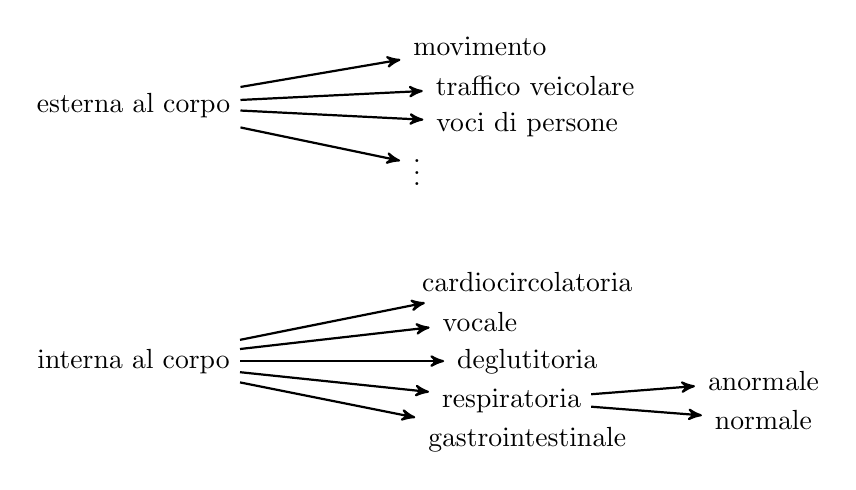
\begin{tikzpicture}    [->,>=stealth',shorten >=1pt,auto,node distance=3cm,
      thick,main node/.style={circle,fill=blue!20,draw,font=\sffamily\Large\bfseries}]
    %   [scale=.8,auto=left,every node/.style={fill=blue!20}]
%       \node (sorgente) at (0,2.625) {sorgente};
    
      \node (interna) at (0,1) 		{interna al corpo};
      \node (esterna) at (0,4.25) 	{esterna al corpo};
    
      \node (respiratoria) at (4.8,0.5) 		{respiratoria};
      \node (gastrointestinale) at  (5,0)	{gastrointestinale};
      \node (deglutitoria) at (5,1) 		{deglutitoria};
      \node (vocale) at (4.4,1.5) 		{vocale};
      \node (cardiocircolatoria) at (5,2) 	{cardiocircolatoria};
    
      \node (vdots) at (3.6,3.5) 	{$\vdots$};
      \node (voci) at (5,4) 		{voci di persone};
      \node (traffico) at (5.1,4.5) 	{traffico veicolare};
      \node (movimento) at (4.4,5)	{movimento};
      
      \node (normale) at (8,0.25) 		{normale};
      \node (anormale) at (8,0.75) 		{anormale};



      \foreach \from/\to in {interna/respiratoria,interna/gastrointestinale,interna/deglutitoria,interna/vocale,interna/cardiocircolatoria,
	  esterna/traffico,esterna/voci,esterna/movimento,esterna/vdots,
	  respiratoria/normale, respiratoria/anormale}
	\draw (\from) -- (\to);
    
    \end{tikzpicture}
  \end{center}
\end{frame}


\begin{frame}[t]
  \frametitle{Caratteristiche del segnale di input\footnote{\emph{Breath Analysis of Respiratory Flow using Tracheal Sounds.} Saiful Huq, Azadeh Yadollahi, Zahra Moussavi. 2007 IEEE International Symposium on Signal Processing and Information Technology}}
  \framesubtitle{Valutazione sperimentale in assenza di rumore esterno}
\begin{center}
\begin{figure}
 \includegraphics[width=\textwidth]{./ba2.png}
 % ba.png: 600x580 pixel, 72dpi, 21.16x20.46 cm, bb=0 0 600 580
\end{figure}
\end{center}
\end{frame}

% \begin{frame}
%   \frametitle{Caratteristiche del segnale di input\footnote{\emph{Breath Analysis of Respiratory Flow using Tracheal Sounds.} Saiful Huq, Azadeh Yadollahi, Zahra Moussavi. 2007 IEEE International Symposium on Signal Processing and Information Technology}}
%   \framesubtitle{Valutazione sperimentale}
% 
% % e anche altri studi (alcuni dei quali citati nella tesi) che usano metodi simili e arrivano a conclusioni simili
% 
% \begin{tikzpicture}[<->,>=stealth',shorten >=1pt,auto,node distance=3cm,
%   thick,main node/.style={fill=none,font=\large\sffamily}]
% 
%   \node[main node] (1) at (0,0) {intensit\`a del suono respiratorio};
% %   \node[main node] (5) at (0,0) {filtrato};
% %   \node[main node] (6) at (0,0.25) {senza rumore};
%   \node[main node] (4) at (2,2) {flusso respiratorio}; % flusso di un solo vettore!
% %   \node[main node] (2) [above left  of=4] {spirometro};
% %   \node[main node] (3) [above right of=1] {microfono};
% 
% 
%   \draw[every node/.style={font=\sffamily\small}]
% %     (1) edge node [left] {direttamente proporzionale} (4)
%       (1) edge node [right] {proporzionale} (4);
% %   \draw[every node/.style={font=\sffamily\small}, ->]
% %       (3) edge node [left] {misura} (1)
% %       (2) edge node [right] {misura} (4);
% %         edge [bend right] node[left] {0.3} (2)
% %         edge [loop above] node {0.1} (1)
% %     (2) edge node [right] {0.4} (1)
% %         edge node {0.3} (4)
% %         edge [loop left] node {0.4} (2)
% %         edge [bend right] node[left] {0.1} (3)
% %     (3) edge node [right] {0.8} (2)
% %         edge [bend right] node[right] {0.2} (4)
% %     (4) edge node [left] {0.2} (3)
% %         edge [loop right] node {0.6} (4)
% %         edge [bend right] node[right] {0.2} (1);
% % ;
% \end{tikzpicture}

% In questo studio gli autori studiano le differenze che ci sono tra la fase inspiratoria e la fase espiratoria in due quantit\`a relative ad un segnale tracheale filtrato con un filtro passa banda. 
% Queste due quantit\`a sono la media e la varianza logaritmica dell'energia. 
% Lo studio usa uno spirometro con pneumotacografo per misurare il flusso. 
% Il flusso viene diviso in base al valore assoluto in: basso, medio, alto e molto alto. 
%\paragraph{input}
%       I dati presi in input sono delle registrazioni di suoni tracheali registrati su nove soggetti sani e non fumatori i quali non hanno mai avuto gravi malattie respiratorie. 
%       Inoltre lo studio aveva a disposizione anche il flusso d'aria registrato attraverso uno spirometro con pneumotacografo
%     \paragraph{algoritmo}
%       L'algoritmo ha due flussi di esecuzione indipendenti, il primo \`e il seguente:
%       \begin{enumerate}
% 	\item 
% 	  Filtro passa alto con frequenza di taglio di $70Hz$ per rimuovere il rumore a bassa frequenza.
% 	\item
% 	  Nelle fasi seguenti l'algoritmo considera solo le porzioni del suono registrate quando il segnale del flusso era al di sotto del $20\%$ del flusso medio o al di sopra del $20\%$ di esso.
% 	  Perch\'e in queste condizioni il suono tracheale si pu\`o considerare stazionario.
% 	\item
% 	  Lo spettro di potenza dei suoni della trachea \`e stato calcolato in una finestra di $50ms$ ($512$ campioni) con il $75\%$ di sovrapposizione tra finestre successive. 
% 	  Per ogni fase respiratoria durante la quale c'era un diverso flusso d'aria, \`e stata calcolata la media della potenza dei suoni tracheali in decibel  entro sei predefinite bande di frequenza: da $70$ a $300Hz$, da $300$ a $450Hz$, da $450$ a $600Hz$, da $600$ a $800Hz$, da $800$ a $1000Hz$ e da $1000$ a $1200Hz$. 
% 	\item
% 	  Dato che le intensit\`a dei suoni respiratori variano da soggetto a soggetto, per ogni soggetto i valori calcolati in precedenza sono stati normalizzati rispetto al valore massimo.
% 	\item
% 	  Si \`e poi calcolata la media dei valori normalizzati tra soggetti diversi per ogni fase respiratoria, inoltre sono state calcolate la media e l'errore standard per diversi tassi di flusso e intervalli di frequenza.
%       \end{enumerate} 
%       mentre il secondo flusso di esecuzione \`e:
%       \begin{enumerate}
% 	\item
% 	  Il segnale dei suoni della trachea sono stati filtrati attraverso un filtro passa alto nelle stesse frequenze menzionate in precedenza. 
% 	\item
% 	  Il segnale filtrato \`e stato in seguito segmentato in finestre di dimensione $50ms$ ($512$ campioni) con il $75\%$ di sovrapposizione tra finestre successive usando una finestra di Hanning. 
% 	\item
% 	  Si calcola il logaritmo della varianza dei segmenti precedenti.
% 	\item
% 	  In ciascuna finestra il valore precedente viene normalizzato rispetto al valore massimo per ridurre le interferenze dei suoni del cuore
% 	\item	
% 	  In seguito viene calcolata la media all'interno delle diverse bande di frequenza e diversi valori del flusso d'aria.
%       \end{enumerate}
%     
%     \paragraph{conclusioni}
%       % \begin{figure}
% 	%  \centering
% 	%  \includegraphics[width=0.9\textwidth]{../Dropbox/tesi respiro/articoli stato dell'arte 1/Breath Analysis of Respiratory Flow using Tracheal Sounds Figura.png}
% 	%  % Breath Analysis of Respiratory Flow using Tracheal Sounds Figura.png: 953x548 pixel, 72dpi, 33.62x19.33 cm, bb=0 0 953 548
% 	%   \label{baorfutsf}
% 	%   
%       % \end{figure}
%       % medium and high flow rate samples of the recorded flow signal along with the spectrogram of the corresponding tracheal sound signal, the normalized logvariance and the normalized Pave over [300-450] Hz.  
%       % It should be noted that the positive (negative) values of the recorded flow signal are related to the inspiratory (expiratory) phases of the respiration cycle. 
%       Da una analisi dello spettrogramma dei suoni tracheali, si pu\`o vedere che l'intensit\`a del suono tracheale aumenta con l'aumentare del valore assoluto del flusso. 
%       Inoltre anche la varianza logaritmica normalizzata e la media di potenza normalizzata seguono i cambiamenti nel valore assoluto del flusso. 
%       Nello spettrogramma, nella varianza logaritmica normalizzata e nella media normalizzata della potenza sono evidenti le transizioni di fase respiratoria. 
%       Quando il flusso era medio o alto, si ha una maggiore differenza di media dell'energia normalizzata tra la fase inspiratoria ed espiratoria nella banda di frequenze dai $300$ ai $450Hz$. 
%       Inoltre questa banda di frequenza ottiene la seconda maggior differenza di media dell'energia normalizzata tra la fase inspiratoria e la fase esipiratoria quando il flusso \`e basso o molto alto. 
%       Quindi questo intervallo di frequenza \`e stato scelto come ottimale per esaminare i cambiamenti nella media della potenza rispettivamente alle fasi respiratorie.
% 
%   





% Lo tolgo questo frame?

% \begin{frame}
%    \frametitle{Caratteristiche del segnale di input}
%   \framesubtitle{Valutazione sperimentale 2}
% \begin{tikzpicture}[<->,>=stealth',shorten >=1pt,auto,node distance=3cm,
%   thick,main node/.style={fill=none,font=\sffamily}]
% 
%   \node[main node] (1) at (0,0.5) {varianza della dimensione};
%   \node[main node] (2) at (0,0.2) {frattale};
%   \node[main node] (3) at (7,0.5) {cambiamento di segno nel}; 
%   \node[main node] (4) at (7,0.2) {flusso respiratorio};
% 
% 
% 
%   \draw[every node/.style={font=\sffamily\small}]
% %     (1) edge node [left] {direttamente proporzionale} (4)
%       (1) edge node [above] {proporzionale} (3);
% %   \draw[every node/.style={font=\sffamily\small}, ->]
% %       (3) edge node [left] {misura} (1)
% %       (2) edge node [right] {misura} (4)
% %         edge [bend right] node[left] {0.3} (2)
% %         edge [loop above] node {0.1} (1)
% %     (2) edge node [right] {0.4} (1)
% %         edge node {0.3} (4)
% %         edge [loop left] node {0.4} (2)
% %         edge [bend right] node[left] {0.1} (3)
% %     (3) edge node [right] {0.8} (2)
% %         edge [bend right] node[right] {0.2} (4)
% %     (4) edge node [left] {0.2} (3)
% %         edge [loop right] node {0.6} (4)
% %         edge [bend right] node[right] {0.2} (1);
% % ;
% \end{tikzpicture}
% 
% \end{frame}





\begin{frame}
  \frametitle{Caratteristiche del segnale di input}
  \framesubtitle{Valutazione anatomico funzionale}
  \begin{itemize}
    \item Origine anatomico funzionale dei suoni respiratori
%     come vengono prodotti i suoni respiratori!!!
    \item Osservazione chiave:
      \textcolor{red}{L'apnea c'\`e quando il flusso \`e zero}
  \end{itemize}
\end{frame}



\section{Implementazione}
\subsection{Estrarre i suoni respiratori dal segnale}
\begin{frame}
  \frametitle{Estrarre i suoni respiratori dal segnale}
  \framesubtitle{Pattern pipeline}
\begin{center}
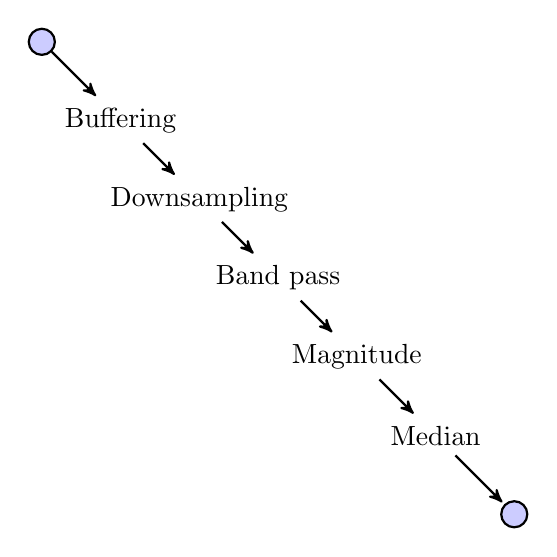
\begin{tikzpicture}
%   [scale=.8,auto=left,every node/.style={fill=blue!20}]
[->,>=stealth',shorten >=1pt,auto,node distance=3cm,
  thick,main node/.style={circle,fill=blue!20,draw,font=\sffamily\LARGE\bfseries}]

  \node [main node] (start) at 		(0,6) 	{};
  \node (Buffering) at 			(1,5) 	{Buffering};
  \node (Downsampling) at 		(2,4)	{Downsampling};
  \node (Band) at 			(3,3) 	{Band pass};
  \node (Magnitude) at 			(4,2) 	{Magnitude};
  \node (Median) at 			(5,1) 	{Median};
  \node [main node] (end) at 		(6,0) 	{};	

   \foreach \from/\to in {start/Buffering,Buffering/Downsampling,Downsampling/Band,Band/Magnitude,Magnitude/Median,Median/end}
     \draw (\from) -- (\to);

\end{tikzpicture}
\end{center}
\end{frame}

% 	Il segnale attraversa la successione di fasi a cascata rappresentate nella figura \ref{filterActivity}. 
% 	Ogni filtro \`e implementato in modo simile a quanto specificato dall'interfaccia $InputStream$ di Java. 
% 	Siamo davanti ad un tipico caso di design di tipo \emph{pipeline} in quanto l'output di un filtro \`e l'input del filtro successivo(eccetto che per l'ultimo filtro). 
% 	Il segnale audio, anche nel caso in cui venga letto da un file, \`e trattato come uno \emph{stream} di dati. 
% 	Pi\`u in dettaglio le fasi di filtraggio sono le seguenti:
%       \paragraph{$Buffering/Windowind$}
% 	Questa fase \`e necessaria in quanto alcuni dei filtri successivi lavorano su blocchi di input e non sul singolo campione. 
% 	Inoltre la presenza del buffer pu\`o diminuire il tempo totale di elaborazione.
% 	In questo caso l'input \`e letto da un file quindi non ci sono problemi di overflow.
% 	Una condizione sufficiente affinch\`e il software rispetti i propri requisiti real time \`e che la velocit\`a di elaborazione sia sempre maggiore di: un secondo di segnale fratto un secondo di tempo di elaborazione. 
%       \paragraph{$Downsampling$}
% 	La sequenza di campionamento viene ridotta con lo scopo di aumentare l'efficienza delle fasi successive dell'algoritmo. 
% 	Gli spettri di potenza dei suoni respiratori e dei suoni cardiaci hanno frequenze al di sotto dei $500Hz$. 
% 	Quindi si pu\`o abbassare la frequenza di campionamento a $1000Hz$ in quanto una larghezza di banda di $500Hz$ \`e adeguata a catturare i suoni respiratori\cite{ASPODUOCSS}. 
%       \paragraph{$Bandpass filtering$}
% 	Questo filtro lascia passare solo i suoni che si trovano nella banda di frequenza dai $100$ ai $1500Hz$, il risultato \`e un suono nel quale sono pi\`u facilmente distinguibili i suoni normali della respirazione. 
% 	Inoltre questo filtro elimina anche alcuni suoni respiratori anormali e parte dei suoni cardiocircolatori.
% 	Questo filtro \`e implementato grazie alle librerie JSTK reperite all'indirizzo \cite{jstk}. 
% 	JSTK sta per Java speech toolkit e fornisce tra le altre cose una libreria di tecniche usate per il riconoscimento vocale. 
% 	La libreria \`e rilasciata secondo la licenza GPLv3.
%       \paragraph{$Magnitude filtering$}
% 	Questo filtro semplicemente prende il valore assoluto del segnale.
%       \paragraph{$Median filtergin$}
% 	Questo \`e un classico filtro a mediana con finestra rettangolare di dimensione $10ms$ e serve per smorzare i suoni accidentali che hanno una intensit\`a relativamente alta rispetto al suono respiratorio e una durata relativamente bassa rispetto alla durata delle fasi respiratorie.

\subsection{Riconoscimento delle apnee}
\begin{frame}
  \frametitle{Riconoscimento delle apnee}
%   \framesubtitle{Pattern pipeline}
\begin{center}
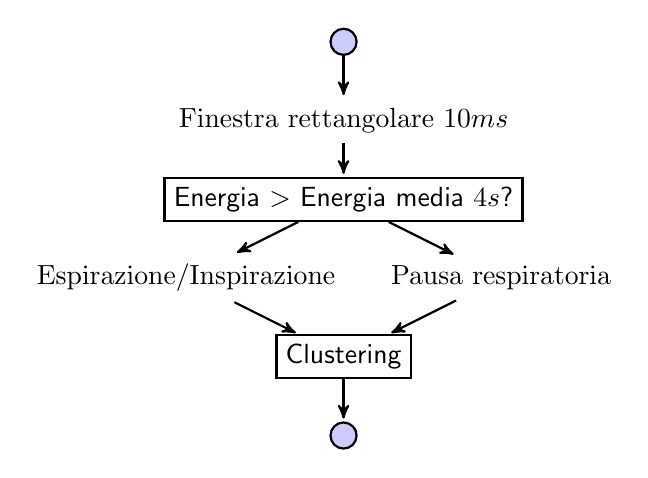
\begin{tikzpicture}
%   [scale=.8,auto=left,every node/.style={fill=blue!20}]
[->,>=stealth',shorten >=1pt,auto,node distance=3cm,
  thick,main node/.style={circle,fill=blue!20,draw,font=\sffamily\LARGE\bfseries},
  decision node/.style={draw,font=\sffamily}]

  \node [main node] (start) at 			(2,5) 	{};
  \node  (Finestra) at 				(2,4) 	{Finestra rettangolare $10ms$};
  \node [decision node] (decision) at 		(2,3)	{Energia $>$ Energia media $4s$?};
  \node (Pausa) at 				(4,2) 	{Pausa respiratoria};
  \node (Espirazione) at 			(0,2) 	{Espirazione/Inspirazione};
  \node [decision node] (Clustering) at	(2,1) 	{Clustering};
  \node [main node] (end) at 			(2,0) 	{};	

   \foreach \from/\to in {start/Finestra,Finestra/decision,decision/Pausa,decision/Espirazione,Pausa/Clustering,Espirazione/Clustering,Clustering/end}
     \draw (\from) -- (\to);

\end{tikzpicture}
\end{center}
\end{frame}

\section{Dettagli implementativi}
\begin{frame}
  \frametitle{Dettagli implementativi}
\begin{center}
  \begin{tabular}{l l}
      \textcolor{blue}{Linguaggio}
    &
      Java
    \\\hline
      \textcolor{blue}{Ambiente di sviluppo}
    &
      Eclipse
    \\\hline
      \textcolor{blue}{Librerie}
    &
      JSTK
%     \\\\
%     \multicolumn{2}{l}{Deploy e test}  
    \\\\\\

	\textcolor{blue}{Calcolatore}
      &
	Laptop Hp Pavilion g6
      \\\hline
	\textcolor{blue}{Microprocessore}
      &
	Intel Core $i3-2330M$ da $2,2GHz$
      \\\hline
	\textcolor{blue}{Cache microprocessore}
      &
	$3 MB$ di cache $L3$
      \\\hline
	\textcolor{blue}{Memoria}
      &
	$DDR3$ da $6 GB$
  \end{tabular}
\end{center}

    

\end{frame}


\section{Test}
\begin{frame}
  \frametitle{Creare i casi di test}
  \begin{itemize}
    \item
      Approccio black box. 
    \item
      Analisi dello spazio dell'input e degli scenari di uso reale.
    \item
      Concatenazione di segmenti di file audio:
% 
% Per la scelta dei casi di test usiamo un approccio di tipo black-box e quindi esaminiamo da prima lo spazio dell'input e poi i possibili scenari di uso. 
% Il tipo dell'input \`e l'insieme di tutti i possibili segnali audio di durata arbitraria.
% Lo spazio dell'input \`e un sottoinsieme del tipo dell'input nel quale rientrano tutti i segnali audio che possono essere ascoltati da uno stetoscopio elettronico posizionato sul petto di un soggetto.
% 
%     \`E possibile individuare alcune classi di suoni nello spazio dell'input in base alle sorgenti:
%     \begin{center}
%     \begin{tikzpicture}
%     %   [scale=.8,auto=left,every node/.style={fill=blue!20}]
%     [->,>=stealth',shorten >=1pt,auto,node distance=3cm,
%       thick,main node/.style={circle,fill=blue!20,draw,font=\sffamily\Large\bfseries}]
%       \node (sorgente) at (0,3) {sorgente};
%     
%       \node (interna) at (4,1.5) {interna al corpo};
%       \node (esterna) at (4,4) {esterna al corpo};
%     
%       \node (n1n1n1) at (9,0) {respiratoria};
%       \node (n1n1n2) at (9,0.5) {muscolare};
%       \node (n1n1n3) at (9,1) {gastrointestinale};
%       \node (n1n1n4) at (9,1.5) {deglutitoria};
%       \node (n1n1n5) at (9,2) {vocale};
%       \node (n1n1n6) at (9,2.5) {cardiocircolatoria};
%     
%       \node (n2n1n3) at (9,3.5) {$\vdots$};
%       \node (n2n1n2) at (9,4) {voci di persone};
%       \node (n2n1n1) at (9,4.5) {traffico veicolare};
%       
%     
%       \foreach \from/\to in {
% 	  sorgente/interna,sorgente/esterna,
% 	  interna/n1n1n1,interna/n1n1n2,interna/n1n1n3,interna/n1n1n4,interna/n1n1n5,interna/n1n1n6,
% 	  esterna/n2n1n1,esterna/n2n1n2,esterna/n2n1n3}
% 	\draw (\from) -- (\to);
%     
%     \end{tikzpicture}
%     \end{center}
% 
% 
% Alcuni casi di test ci vengono dati dai possibili valori che pu\`o avere l'input in uno scenario di uso reale del software. Ad esempio alcuni casi di test possono avere come input:
% \begin{itemize}
%   \item
%     Un file audio abbastanza lungo da simulare un monitoraggio del sonno reale. Lo scopo di un caso d'uso con questo input \`e la valutazione della velocit\`a a lungo termine dell'algoritmo.
%   \item
%     Dei suoni respiratori sovrapposti a rumore di vari tipo ed intensit\`a. Lo scopo di un caso d'uso con questo input \`e la valutazione della tolleranza al rumore.
%   \item
%     Suoni respiratori senza rumore. Lo scopo di un caso d'uso con questo input \`e la valutazione del funzionamento del software in uno scenario ideale.
%   \item
%     Un file audio contenente solo rumore. Questo caso di test serve per capire se il software pu\`o rilevare la presenza di respiro in suoni che non contengono alcun respiro. In uno scenario di uso reale corretto questo caso non si verifica ma \`e comunque interessante.
%   \item
%     Un file con una frequenza di campionamento molto elevata. Questo caso di test rientra nella categoria stress test. Ci aspettiamo che il sistema si comporti bene se ha un input file con una frequenza di campionamento molto elevata grazie al filtro di sottocampionamento.
%   \item
%     Un file contenente suoni respiratori sovrapposti a forti suoni cardiaci. 
%   \item
%     Un file respiratorio contente una apnea pi\`u lunga della soglia massima.
% \end{itemize}
% 
% Per creare dei casi che valutano la resistenza al rumore si pu\`o procedere nel modo illustrato nella figura \ref{mix} e cio\`e:
% \begin{enumerate}
%   \item 
%     Scegliere una file contenente una sorgente di rumore e scegliere una intensit\`a della sorgente di rumore.
%   \item
%     Filtrare il file di rumore in base ad un certo modello acustico del corpo. Cio\`e cercare di prevedere cosa lo stetoscopio sente se \`e presente la sorgente di rumore scelta. Questo modello acustico \`e necessariamente un modello approssimato. In una prima fase elementare di modellazione possiamo usare un semplice filtro attenuatore e supporre che il rumore sia di tipo additivo.
%   \item
%     Scegliere un file contente un respiro.
%   \item
%     Fare un mix dei file.
% \end{enumerate}
% 
% 
% \begin{center}
% \begin{figure}
% \centering
% \begin{tikzpicture}[scale=2,->,>=stealth',shorten >=1pt,auto, thick,nodes={draw, ultra thick, fill=none}]
%       
%       \node[draw=none] (respiro) at (0,1) {respiro};
%       \node[draw=none] (rumore) at (0,0) {rumore};
% 
%       \node[rectangle] (attenuatore) at (2,0) {filtro attenuatore};
%       \node[rectangle] (somma) at (2,1) {+};
% 
%       \node[draw=none] (output) at (4,1) {output};
% 
% 
% 
%   \foreach \from/\to in {respiro/somma, rumore/attenuatore, attenuatore/somma, somma/output}
%      \draw (\from) -- (\to);
% 
% \end{tikzpicture}
%   \caption{Processo di aggiunta del rumore}
% \label{mix}
% \end{figure}
% \end{center}
% 
% 
% 
% Arriva in nostro aiuto il software open source Audacity \cite{audacity} il quale offre una vasta gamma di funzioni di trattamento dell'audio digitale. Quelle utili per i casi di test sono: 
% \begin{itemize}
%   \item
%     Aggiungere rumore di vari tipi (bianco, rosa e marrone) e con varia intensit\`a.
%   \item
%     Aggiungere segmenti di silenzio di lunghezza a scelta nei file audio e quindi simulare la presenza di una apnea lunga.
%   \item
%     Concatenare file audio. Questa funzione \`e utile perch\'e i file audio che abbiamo a disposizione reperiti da \cite{SoundRepositories} sono di lunghezza troppo breve (minore di $15s$).
%   \item
%     Applicare filtri di vario tipo tra i quali un filtro attenuatore.
% \end{itemize}
% 
% 

 
 \begin{center}
   \begin{table}[!h]
     \centering
     \begin{tabular}{p{0.15\textwidth} | p{0.5\textwidth} l}
       \hline
 	  contenuto
 	& 
 	  tipo o sorgente
 	& 
 	  itensit\`a
       \\\hline\\
 	  respiro
 	& 
%  	  [normale anormale misto, bronchiale vescicolare, continuo discontinuo, ronchi wheeze stridor crackles squawks]
	  [normale, anormale, misto, bronchiale, vescicolare, continuo, ...]
 	& 
 	  [0-10]
       \\
 	  rumori
 	& 
 	  [bianco, rosa, interno, esterno, gastrointestinale, ...]
 	& 
 	  [0-10]
       \\
 	  pausa respiratoria
 	& 
 	  -
 	& 
 	  -
       \\\hline
     \end{tabular}
   \end{table}
 \end{center}
  \end{itemize} 
% 
% Non abbiamo a disposizione alcuno stetoscopio per\`o usiamo le registrazioni reperite da \cite{SoundRepositories} e partiamo da queste per creare alcuni casi di test.
% Purtroppo le fonti non riportano i dettagli di come sono stati registrati i suoni. 
% 

\end{frame}


\begin{frame}
  \frametitle{Valutazione dell'output}
  \framesubtitle{Localizzazione delle apnee a rischio}
% 
% \section{Valutazione dell'output}
% \label{valutareOutput}
% \paragraph{Valutare la localizzazione delle fasi respiratorie.}
% Se si vuole valutare un algoritmo che localizza nel tempo le fasi respiratorie allora pensiamo ad un suono respiratorio come ad una sequenza di cicli respiratori e ad  un ciclo respiratorio come una fase di inspirazione seguita da una fase di espirazione seguita da una pausa. 
% 
\begin{itemize}
  \item 
    Classificazione dello spazio dell'input: sequenze di intervalli di numeri razionali che indicano la posizione temporale di ciascuna fase di apnea.
  \item
    Classificazione dell'output rispetto alla classe di input:
% Quindi lo spazio di input \`e classificabile in sequenze crescenti di numeri razionali che indicano la posizione temporale dell'inizio di ciascuna fase. L'output dell'algoritmo sar\`a una sequenza di numeri razionali che indicano la localizzazione temporale dell'inizio di ciascuna fase. 
% Definiamo la differenza tra l'output e il descrittore della classe di cui fa parte l'input come la sequenza dei valori assoluti delle differenze delle singole componenti. 
% La qualit\`a dell'algoritmo si pu\`o misurare in termini di qualche propriet\`a statistica di questa differenza, ad esempio la media.
% 
% 
% \paragraph{Valutare la localizzazione delle apnee.}
% Se si vuole valutare un algoritmo che riconosce la presenza di una apnea allora possiamo classificare lo spazio dell'input in sequenze di coppie di numeri razionali tali che ogni coppia contiene il tempo di inizio e il tempo di fine di una apnea. In tal caso anche l'output sar\`a una sequenza di coppie di numeri razionali. 
% Supponiamo che in input ci sia una apnea che comincia al tempo $s_{in}$ e finisce al tempo $f_{in}$. Si possono verificare vari casi:
% \begin{itemize}
%   \item
%     Esiste un solo intervallo temporale di output $(s_{out}, f_{out})$ che interseca l'intervallo $(s_{in}, f_{in})$. Allora definiamo l'errore di riconoscimento dell'evento $(s_{in}, f_{in})$ come 
%     \[
%       |s_{out}-s_{in}| + |f_{out}-f_{in}|
%     \]
%     e diciamo che l'evento $(s_{in}, f_{in})$ \`e un \emph{vero positivo} cio\`e un evento riconosciuto in modo corretto.
%   \item
%     Se non ci sono intervalli temporali di output che intersecano $(s_{in}, f_{in})$ allora diciamo che questo evento \`e un \emph{falso positivo}. I falsi positivi sono gli errori pi\`u gravi e che quindi incidono maggiormente nella valutazione di un algoritmo.
%   \item
%     Se ci sono pi\`u intervalli temporali di output che intersecano $(s_{in}, f_{in})$ allora la scelta di come valutare la qualit\`a dell'algoritmo \`e arbitraria e pu\`o essere ad esempio 
%     \[
%       |min(s_{out})-s_{in}| + |max(f_{out})-f_{in}|
%     \]
% \end{itemize}
% Rimane il caso in cui l'algoritmo produce un output $(s_{out}, f_{out})$ ma non abbiamo nessun intervallo di input che lo interseca. 
% In tal caso parliamo di \emph{falso negativo} ed \`e un errore meno grave di un falso positivo. 
% 
% \paragraph{Valutare la localizzazione delle apnee a rischio.}
% Se si vuole valutare un algoritmo che riconosce la presenza di una apnea troppo lunga allora possiamo classificare lo spazio dell'input come nel caso precedente ma l'analisi che ne risulta \`e diversa.
% Supponiamo che in input ci sia una apnea troppo lunga (cio\`e maggiore di una certa soglia $S$ di sicurezza) che comincia al tempo $s_{in}$ e finisce al tempo $f_{in}$. Si possono verificare vari casi:
% \begin{itemize}
%   \item
%     C'\`e almeno un intervallo temporale di output $(s_{out}, f_{out})$ tale che 
%     \begin{itemize}
%       \item 
% 	$(s_{out}, f_{out})$ interseca $(s_{in}, f_{in})$
%       \item
% 	$s_{out} + S \leq s_{in} + S + T$ dove $T$ \`e una soglia di tolleranza dell'errore.
%       \item
% 	$f_{out}-s_{out}>S$
%     \end{itemize}
%     In tal caso diciamo che l'evento $(s_{in}, f_{in})$ \`e un \emph{vero positivo} cio\`e un evento riconosciuto in modo corretto.
%   \item
%     Se non ci sono intervalli temporali di output con le propriet\`a elencate al punto precedente allora diciamo che l'evento $(s_{in}, f_{in})$ \`e un \emph{falso positivo}.
% \end{itemize}
% Rimane il caso in cui l'algoritmo produce in output un intervallo $(s_{out}, f_{out})$ di lunghezza maggiore della soglia di sicurezza ma non abbiamo nessun intervallo di input che lo interseca e che ha durata maggiore della soglia di sicurezza. 
% In tal caso abbiamo un \emph{falso negativo}. 
% Si pu\`o anche definire cosa intendiamo per \emph{vero negativo} e cio\`e una mancanza di apnea troppo lunga che l'algoritmo non classifica come apnea troppo lunga. 
% Tuttavia questa definizione non si applica in modo elegante alle premesse fatte in questo paragrafo. 
% La tabella seguente ricapitola i vari casi:
 \begin{center}
     \begin{tabular}{|l|ll|}
       \hline
       \emph{apnea troppo lunga} & evento presente & evento assente \\
       \hline
       evento riconosciuto        & \textcolor{green}{vero positivo}   & falso negativo \\
       evento non riconosciuto    & \textcolor{red}{falso positivo}  & \textcolor{green}{vero negativo}  \\
       \hline
     \end{tabular}
\end{center}
\end{itemize}
% 
% Si pu\`o capire facilmente quale significato abbia la classificazione precedente, se si immagina uno scenario di uso del software.
% 
% 
% \begin{bf}Vero positivo.\end{bf}
%   Il soggetto ha una apnea nel sonno troppo lunga e il sistema suona l'allarme. Il soggetto si sveglia, spegne l'allarme e torna a dormire sano e salvo (si spera).
% 
% 
% \begin{bf}Vero negativo.\end{bf}
%   Il soggetto non ha una apnea nel sonno troppo lunga e il sistema non suona l'allarme. Questo caso \`e auspicabile. Maggiore \`e la frequenza di questi casi, maggiore \`e la qualit\`a del sonno del soggetto.
% 
% 
% \begin{bf}Falso positivo.\end{bf}
%   Il soggetto ha una apnea nel sonno troppo lunga e il sistema non suona l'allarme. Questo caso \`e rischioso per la salute del paziente.
% 
% 
% \begin{bf}Falso negativo.\end{bf}
%   Il soggetto non ha una apnea nel sonno troppo lunga e il sistema suona l'allarme. Il soggetto si sveglia, spegne l'allarme e torna a dormire. Non ha modo di capire se si \`e verificato un vero positivo o un falso negativo (quindi non impreca contro gli sviluppatori del software).
%     I falsi negativi degradano la qualit\`a del sonno del soggetto ma non sono un rischio grave per la salute quanto i falsi positivi.
%     Tuttavia se il degrado nella qualit\`a del sonno \`e eccessivo potrebbe causare danni psicofisici al soggetto che eventualmente superano quelli causati dalla sindrome da apnea del sonno.
%     Quindi \`e anche importante che il sistema non generi molti falsi negativi.


    

\end{frame}


\begin{frame}
  \frametitle{Risultati dei test}
  \framesubtitle{Casi di test sulle registrazioni}

%   \section{Casi di test e risultati}
%     I test fatti sono di tipo \emph{oracolo} nel senso che l'output dell'algoritmo in ogni caso di test viene confrontato con il risultato che l'algoritmo dovrebbe fornire. 
%     I test sono stati fatti su un laptop \emph{Hp Pavilion g6} con le seguenti caratteristiche:
%     \begin{center}
%       \begin{table}[!h]
%       \centering
%       \begin{tabular}{l|l}
% 	Microprocessore
%       &
% 	Intel Core $i3-2330M$ da $2,2GHz$
%       \\\hline
% 	Cache microprocessore
%       &
% 	$3 MB$ di cache $L3$
%       \\\hline
% 	Memoria
%       &
% 	$DDR3$ da $6 GB$
%     \end{tabular}
%     \caption{Caratteristiche del calcolatore usato per i test.}
%     \end{table}
%   \end{center}
% 
%   \subsection{Casi di test sui file delle repository}
%     I file usati in questo caso di test sono descritti in una sezione successiva \ref{repoDesc}.
%      In seguito all'ascolto e alla visualizzazione della forma d'onda dei file, si nota che nessuno dei file contiene una apnea troppo lunga.
%      La tabella \ref{esitoRepository} riporta nell'ordine: il nome del file, il tempo di esecuzione totale dell'algoritmo  e un errore approssimato nella localizzazione delle apnee.
%      Il tempo di esecuzione dell'algoritmo \`e espresso come media dei tempi di esecuzione per secondo di segnale. 
 \begin{table}
   \begin{tabular}{|l  p{0.18\textwidth}  p{0.5\textwidth} |}
\hline
   File (.wav)						&Tempo di esecuzione		&Errore nella localizzazione di apnee non a rischio\\
 \hline\hline
   Coarse crackles					&$2ms$			&$0.4s$	pi\`u un falso negativo		  \\
\hline
   Normal vesicular	 				&$14ms$			&$0.2s$	 \\
\hline
   Pleural friction					&$3ms$			&$0.4s$ pi\`u $2$ falsi negativi	\\
\hline
   Inspiratory stridor					&$3ms$			&
%   
 \vspace{-4mm}
\begin{itemize}
   \item 	
    riconosce la fine delle pause e l'inizio delle inspirazioni con un margine di errore di $0.4s$ 
   \item 	
    confonde le espirazioni con una pausa perch\'e queste hanno intensit\`a molto bassa			  					  
\end{itemize}
\vspace{-4mm}

\\
   \hline
   \end{tabular}
 \end{table}

\end{frame}

\begin{frame}
  \frametitle{Risultati dei test}
  \framesubtitle{Caso di test di localizzazione di una apnea troppo lunga}
% AGGIUNGERE NELLA TABELLA PRECEDENTE!
 
%  \subsection{Caso di test di localizzazione di una apnea troppo lunga}
\begin{itemize}
  \item
    Apnea aggiunta con Audacity dall'istante $35s$ all'istante $1m:17s$. 
  \item
    Apnea riconosciuta in modo corretto dall'istante $36s$ all'istante $1m:16s$.
  \item
    L'allarme suona all'istante $66s$ cio\`e $30s$ dopo l'inizio della pausa.
\end{itemize}

%  In questo caso di test prendiamo il file normal.wav reperito da \cite{SoundRepositories}, che contiene un respiro normale di un soggetto sano, lo concateniamo varie volte e aggiungiamo con Audacity una pausa respiratoria molto lunga. 
%  La pausa comincia al tempo $35s$ e termina al tempo $1h:17s$. 
%  La lunghezza totale del file \`e $1h:41s$.
%  Il sistema riconosce in modo corretto la pausa dal tempo $35s$ al tempo $1h:15s$.
%  L'allarme suona al tempo $63s$ cio\`e $30s$ dopo l'inizio della pausa, e questo \`e esattamente quello che ci aspettiamo.
%  Quindi possiamo dire che questo caso di test si \`e concluso con successo.
% 
% 
% 
% 
% 
% \section{Descrizione dei file di respiro reperiti da \cite{SoundRepositories}}
% \label{repoDesc}
%     La tabella \ref{descrizioneRepo} seguente riporta una descrizione di alcuni dei file reperiti da \cite{SoundRepositories}. 
%     Le colonne della tabella riportano nell'ordine: nome del file, durata del file, classificazione dei suoni respiratori contenuti nel file e infine frequenza di respirazione espressa in cicli di respirazione al secondo. 
%     La frequenza di campionamento di tutti i file (espressa in numero di campioni al secondo) \`e di $8000 Hz$ e lo schema di respirazione \`e normale.
%     
% \begin{table}
%   \begin{tabular}{l l l p{0.43\textwidth}}
%   \hline
%       Nome file 
%     &
%       Durata
%     &
%       Frequenza
%     &
%       Classificazione dei suoni respiratori
%   \\\hline\\
%       Coarse crackles.wav
%     &
%       $12s$
%     &
%       $25/60 Hz$
%     &
%       Normali e presenza di crackles
%   \\
%       Normal vesicular.wav
%     &
%       $13s$
%     &
%       $13.8/60 Hz$
%     &
%       Normali
%  \\
%       Inspiratory stridor.wav
%     &
%       $14s$
%     &
%       $21/60 Hz$
%     &
%       Normali e presenza di stridor durante la fase inspiratoria
%   \\
%       Pleural friction.wav
%     &
%       $20s$
%     &
%       $18/60 Hz$
%     &
%       Normali e presenza di frizione pleurica. Il suono \`e molto rumoroso e non \`ed \`e difficile distinguere le fasi respiratorie.
%       
%   \\\hline
%   \end{tabular}
%   \caption{Descrizione dei file delle repository.}
%   \label{descrizioneRepo}
% \end{table}
% 
% 
% 
% 
% 
% 
% 
\end{frame}




\begin{frame}
  \frametitle{Risultati dei test}
  \framesubtitle{Resistenza al rumore bianco}
Se il rumore bianco ha una intensit\`a che supera il $30\%$ dell'intensit\`a massima dei suoni respiratori allora il sistema non riconosce nessuna pausa respiratoria.
  \begin{figure}
 \centering
 \includegraphics[width=0.9\textwidth]{./testWhiteNoise.png}
 % testWhiteNoise.png: 616x322 pixel, 72dpi, 21.73x11.36 cm, bb=0 0 616 322
\end{figure}
% \subsection{Caso di test di tolleranza al rumore bianco}
% Il protagonista di questo caso di test \`e il file Normal vesicular.wav che contiene un suono respiratorio normale disturbato da un rumore leggero. A questo file aggiungiamo con Audacity del rumore bianco di intensit\`a crescente e valutiamo le prestazioni del sistema. Il file ha le seguenti caratteristiche:
% \begin{itemize}
%  \item 
%     L'intensit\`a massima \`e circa $0.2dB$.
%   \item
%     L'intensit\`a media delle fasi inspiratorie \`e circa $0.08dB$.
%   \item
%     L'intensit\`a media delle fasi di pause respiratorie \`e circa $0.02dB$.
% \end{itemize}
% 
% L'intensit\`a del rumore aggiunto va da $0dB$ a $0.2dB$ con un incremento di $0.02dB$, quindi eseguiamo $11$ test. 
% In nessun caso era presente una apnea troppo lunga e in nessun caso l'algoritmo ha rilevato la presenza di una apnea troppo lunga quindi dal punto di vista del riconoscimento di apnee troppo lunghe, l'algoritmo funziona in modo corretto. 
% \`E comunque interessante valutare l'output dell'algoritmo con un maggior livello di dettaglio. 
% La figura \ref{testNormalWhiteNoise} illustra una rappresentazione dell'output dell'algoritmo sui file di test e contiene un grafico per ogni file di input.
% \begin{figure}
%  \centering
%  \includegraphics[width=0.9\textwidth]{./testWhiteNoise.png}
%  % testWhiteNoise.png: 1366x768 pixel, 72dpi, 48.19x27.09 cm, bb=0 0 1366 768
%   \caption{Risultati del test di tolleranza al rumore bianco.}
%   \label{testNormalWhiteNoise}
% \end{figure}
% 
% I valori sulle ascisse segnano il tempo in decimi di secondo.
% I grafici contenuti nella figura dal basso verso l'alto escluso il primo sono relativi a file che hanno una quantit\`a di rumore crescente e mostrano quali parti dei rispettivi file vengono riconosciuti come respiro e quali parti vengono riconosciuti come apnea.
% Invece il primo grafico in basso rappresenta il file originale in termini di fasi di respiro e fasi di pausa, stimate da un ascolto del file.
% I valori di questo grafico sono approssimativi e non \`e possibile ottenere valori pi\`u precisi se non si misura il flusso d'aria in modo diretto.
% Notiamo che gli ultimi $7$ grafici dal basso sono semplicemente dei segmenti di retta, questo perch\`e l'algoritmo riconosce l'intero file come respirazione cio\`e non riconosce alcuna pausa. 
% Mentre nei primi $5$ grafici dal basso il segmento di retta pu\`o essere in basso ad indicare una pausa oppure in alto ad indicare la presenza di una inspirazione o di una espirazione.
% 
% 
% % Nel grafico in figura \ref{graficoCasoDiTestRumoreBianco}, l'asse delle ascisse riporta la quantit\`a di rumore bianco aggiunto in termini di percentuale di decibel di rumore rispetto all'intensit\`a massima del respiro, mentre l'asse delle ordinate riporta l'errore calcolato in base a quanto detto nella sottosezione \ref{valutareOutput}.

\end{frame}








\section{Sviluppi futuri}
\begin{frame}
\frametitle{Sviluppi futuri}

\begin{itemize}
  \item 
    Classificare i suoni respiratori (normali, anormali, soffi, crackles, ...).
  \item
    Riconoscere gli schemi respiratori (normale, Cheyne Stokes, agonico, Kussmaul, ...).
  \item
    Implementare un'interfaccia con uno stetoscopio elettronico.
  \item
    Implementare un algoritmo di stima del flusso.
  \item
    Portare il software su un dispositivo mobile. 
  \item
    Creare un database di registrazioni di suoni respiratori.    
  \item
    Creare un database di casi di test.
  \item
    Implementare dei meccanismi di tolleranza al rumore esterno. Ad esempio attraverso la creazione di un modello acustico approssimato del torace.
\end{itemize}

% 	
% 	Ad esempio usare due microfoni: uno che registra il rumore ambientale e uno che registra i suoni respiratori e usare il modello acustico per estrarre il rumore ambientale dai suoni respiratori.
%       \item
% 	Fare una analisi approfondita dello stato dell'arte della separazione dei suoni cardiovascolari dai suoni respiratori, partendo ad esempio dagli articoli \cite{separazione1, separazione2, separazione3, separazione4, separazione5, separazione6}.
%     \end{itemize}
\end{frame}









\section{Conclusioni}
\begin{frame}
\frametitle{Conclusioni}
% \framesubtitle{Commenti}


\begin{description}
  \item[Obiettivi]
    Progettare, prototipare e valutare un software di riconoscimento delle apnee notturne attraverso uno stetoscopio elettronico applicato sul petto o sulla trachea di un soggetto.
  \item[Risultati] 
    I risultati raggiunti sono incoraggianti e
    fanno da un punto di partenza verso un sistema usabile in uno scenario reale.    
\end{description}

% Gli obbiettivi di questa tesi sono di progettare, prototipare e valutare un software di riconoscimento delle apnee notturne attraverso uno stetoscopio elettronico applicato sul petto o sulla trachea di un soggetto.
%  Ricapitolare quello che e' stato fatto. ricordare qual'era l'obbiettivo, dire che il sistema e' stato implementato e testato con risultati incoraggianti




\end{frame}


\end{document}









